\documentclass[10pt,a4paper]{article}
\usepackage[utf8]{inputenc}
\usepackage[russian]{babel}
\usepackage[OT1]{fontenc}
\usepackage{amsmath}
\usepackage{amsfonts}
\usepackage{amssymb}
\usepackage{makeidx}
\usepackage{graphicx}

\usepackage{graphicx}
\usepackage{caption}
\usepackage{subcaption}

\usepackage{float}
\floatstyle{boxed}
\restylefloat{figure}

\author{Максим Борисяк}
\title{Дипломная работа}
\makeindex

\newtheorem{defen}{Определение}

\newcommand{\stock}{\text{STOCK}}
\newcommand{\source}{\text{SOURCE}}

\newcommand{\FA}{F\!A}

%\textheight = 720pt
%\textwidth = 500pt

%\hoffset = -25mm
%\voffset = -30mm

\begin{document}

\maketitle

\section{Введение}

Введение.

\subsection{Мотивация}
Мотивация

\subsection{Базовые понятия и определения}
В данном разделе будут введены базовые понятия, используемые в данной работе, в том числе,
понятия атомарного блока, составного блока, потока данных, автомата Мили соответствующего блоку и так далее.

Основной единицей потока данных является атомарный блок.
\begin{defen}
  \textbf{Шаблоном атомарного блока} $s$ назовем кортеж имеющий два не пересекающихся набора портов: \textit{входной} и \textit{выходной}.
  $s = (\FA, I, O)$, где:
  \begin{itemize}
    \item $I = \{b^I_i \vert i = \overline{1, N_I}, N_I \in \mathbb{N}\}$ --- конечное множество уникальных входных портов;
    \item $O = \{b^O_i \vert i = \overline{1, N_O}, N_O \in \mathbb{N}\}$ --- конечное множество уникальных выходных портов;
    \item $\FA$ --- конечный автомат Мили, смысл и структура которого будет обсуждаться в дальнейшем.
  \end{itemize}
\end{defen}
Сразу заметим, что не любая тройка $(\FA, I, O)$ является шаблоном атомарного блока, так как $\FA$ должен
соответствовать множествам $I$ и $O$.
  
Введем так же функции $inputs(s) = I$ и $outputs(s) = O$ равные множествам входных и выходных портов шаблона блока $s$ соответственно.
Стоит отметить, что природа множеств $O$ и $I$ совершенно не важна, например, они могут быть просто множеством чисел: $I, O = \{i \in \overline{1, \dots, N_{I, O}}\}$,
на практике часто используют строки для именования портов, так как порты могут существенно различаться по смыслу, а их именование помогает избежать путаницы.
Мы будем придерживаться последнего подхода.
  
Для автомата Мили введем функцию $\FA(s) = \FA$ и $S(s) = S$, где $S$ --- множество состояний $\FA(s)$.

\begin{defen}
  \textbf{Атомарным блоком} $b = (id, s, state)$, где:
  \begin{itemize}
    \item $id$ --- уникальный для всех блоков идентификатор;
    \item $s$ --- шаблон атомарного блока;
    \item $state \in S$, где $S$ множество состояний $\FA(s)$ --- текущее состояние атомарного блока.
  \end{itemize}
\end{defen}

Идентификатор $id$ введен из-за следующих соображений: в потоке данных некие блоки могут описываться одним и тем же шаблоном, находиться в одном и том же состоянии,
но все равно будут являться различными блоками, в частности, могут перейти в различные состояния в следующие моменты времени либо могут иметь в потоке данных разный смысл и,
соответственно, иметь различные соединения с другими блоками.

Так же определим функции $state(b) = state$, $id(b) = id$ и перенесем все функции шаблона блока на атомарный блок, например, $\FA(b) = \FA(s)$.

В реальных системах для построения и запуска потока данных шаблон атомарного блока представляется в виде подпрограммы или модуля
(функции, класса некого объектно-ориентированного языка программирования, динамической библиотеки), который используя данные некого набора своих входных портов,
вычисляет и записывает данные в свои выходные порты. В таком случае, атомарный блок представляется в виде набора внутренних переменных,
либо (что тоже самое) в виде экземпляра класса объектно-ориентированного языка программирования соответствующего шаблону.
В такой интерпретации некую вычислимую функцию $f(x_1, x_2, \dots, x_n)$ можно представить в виде шаблона блока $b_f$
с входными портами $x_1, x_2, \dots, x_n$ и одним выходным портом $F$, который при получении данных со всех входных портов
выписывает значения функции $f(x_1, x_2, \dots, x_n)$ в порт $F$.

На рисунке \ref{map} схематично изображен шаблон блока \textit{Loop}, для которого $inputs(Loop) = \{xs, f\}$, $outputs(Loop) = \{fs, x\}$.

\begin{figure}[H]
  \centering

  \begin{subfigure}[b]{0.2\textwidth}
    \centering
    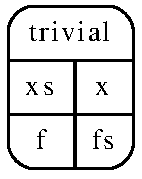
\includegraphics[width=\textwidth]{map_cg.pdf}
    \caption{Схема шаблона \textit{Loop}}
    \label{map:connection}
  \end{subfigure}
  ~
  \begin{subfigure}[b]{0.7\textwidth}
    \centering
    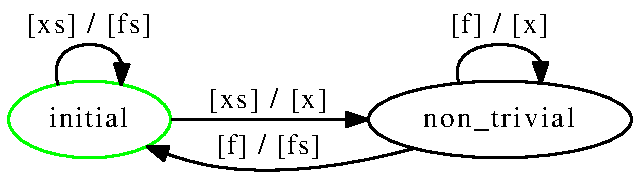
\includegraphics[width=\textwidth]{map_fa.pdf}
    \caption{Автомат Мили шаблона \textit{Loop}}
    \label{map:fa}
  \end{subfigure}
  
  \caption{Схематичное изображение шаблона блока \textit{Loop} (a) и соответствующего ему конечного автомата Мили (b).}
  \label{map}
\end{figure}

Основной структурой для построения схемы потока данных является составной блок.

\begin{defen}
 \textbf{Шаблоном составного блока} будем называть кортеж $c = (B, E, I, O)$, где:
 \begin{itemize}
    \item $B$ - множество блоков (сразу заметим, что блоком может являться и составной блок, определенный ниже).
    \item $E$ - множество ребер вида $e_b = (b_1, b^O_{1}, b_2, b^I_{2})$, $b_1, b_2 \in B$, $b^O_{1} \in outputs(b_1), b^I_{2} \in inputs(b)$,
                либо вида $e_I = (c^I, b, b^I)$, $e_O = (b, b^O, c^O)$, где $b \in B$, $b^I \in inputs(b)$, $b^O \in outputs(b)$, $c^O \in O$, $c^I \in I$.
                Множества ребер $e_b$ будем обозначать как $E^B$, $e_I$ и $e_O$ как $E^I$ и $E^O$ соответственно.
    \item $I$, $O$ - наборы входных и выходных портов (по аналогии с атомарным блоком).
  \end{itemize}
  Аналогично шаблону атомарному блоку определяются функции $inputs(c) = I$ и $outputs(c) = O$.
\end{defen}

Для анализа внутренней структуры удобно рассматривать иное представление шаблона составного блока, добавляя фиктивные блоки $\stock$, $inputs(\stock) = outputs(\stock) = O$,
  и $\source$, $inputs(\source) = outputs(\source) = I$:
$$\hat{E}^I = \{(\source, \source^O, b, b^I) \vert (\source^O, b, b^I) \in E^I\}$$
$$\hat{E}^O = \{ (b, b^O, \stock, \stock^I) \vert (b, b^O, \stock) \in E^O \}$$
$$\hat{c} = (B \cup \{\stock, \source\}, E^B \cup \hat{E}^I \cup \hat{E}^O)$$
В этом случае шаблон составного блока $\hat{c}$ описывается графом с ребрами вида $(u, u^O, v, v^I)$,
а входными и выходными портами всего шаблона считаются входные и выходные порты блоков $\source$ и $\stock$.
На рисунке \ref{example} изображен примеры шаблонов составных блоков.

\begin{defen}
  \textbf{Составным блоком} будем называть $b = (id, c = (B, E, I, O), state)$, где
  \begin{itemize}
    \item $id$ --- уникальный идентификатор;
    \item $c$ --- шаблон составного блока;
    \item $state \in \Sigma \times 2^E = \prod S(B) \times 2^E \times 2^B$ - текущие состояние составного блока, включающее
          состояние каждого блока (подпространство $\Sigma = \prod S(B)$), активную волну ($\omega \in \Omega = 2^E$) и
          множество активных блоков ($\vartheta \in \Theta = 2^B$), смысл которых будет пояснен позже.
  \end{itemize}
\end{defen}

\begin{figure}[H]
  \centering
  \begin{subfigure}[b]{0.3\textwidth}
    \centering
    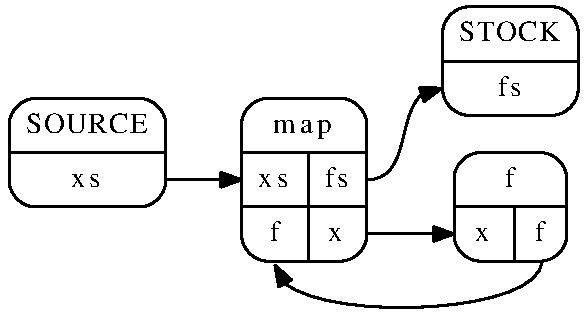
\includegraphics[width=\textwidth]{example_cg.pdf}
    \caption{Шаблон составного блока}
    \label{example:composite}
  \end{subfigure}
  ~
  \begin{subfigure}[b]{1.0\textwidth}
    \centering
    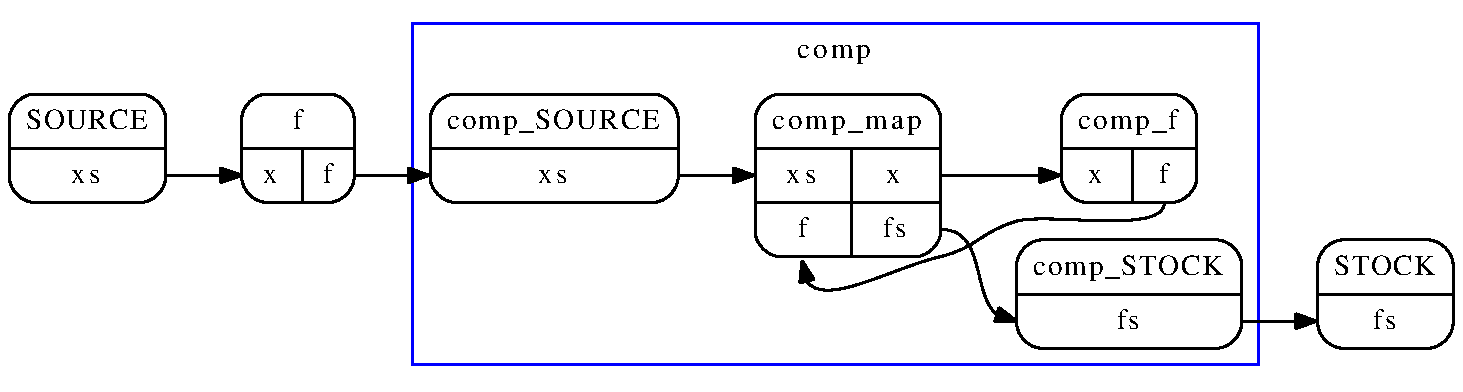
\includegraphics[width=\textwidth]{cc_cg.pdf}
    \caption{Шаблон супер-составного блока. Внутри рамки показана структура шаблона внутреннего блока.}
    \label{example:supercomposite}
  \end{subfigure}
  
  \caption{ Примеры графов составного и супер-составного блока.}
  \label{example}
\end{figure}

Заметим, что составной блок (в исходной интерпретации) внешне не отличим от атомарного блока.
Поэтому под понятием блока мы будем подразумевать либо атомарный блок, либо составной блок,
различая их только в том случае, когда речь заходит о их внутреннем строении. Составной блок может включать в себя другие составные блоки.
На рисунке \ref{example:supercomposite} показан пример составного блока, включающего другой составной блок, иными словами супер-составного блока.
На практике свойство вложенности реализует принцип модульности программ --- модулем в нашем случае будет шаблон составного блока.
Бессмысленно рассматривать случаи, в которых структура составного блока бесконечна в глубину, например,
в случае когда шаблон составного блок содержит содержит блок того же шаблона. Поэтому в дальнейшем, мы будем рассматривать только составные блоки конечной глубины.

Заметим, что составным блоком можно описать любую программу, имея в распоряжении необходимые примитивы --- шаблоны атомарных блоков,
реализующие Тьюринг-полную систему операций. Доказательства этого факта выходит за задачи данной работы и может быть найдено, например, в работе \textbf{[???]}.
Из-за достаточной выразительности составного блока, схему потока данных мы определим просто как схему некого составного блока.

Теперь неформально поясним схему работы составного блока и смысл его структуры.
В общепринятых определениях потока данных ребра графа шаблона составного блока обозначают зависимость по данным, то есть ребро $e = (u, u^O, v, v^I)$ представляет собой
\textit{FIFO}-канал соединения между портами блоков и
можно словесно интерпретировать следующим образом: блок $v$ в качестве данных из входного порта $v^I$ должен использовать данные выходного порта $u^O$ блока $u$ при их наличии.
Блок $u$ после завершения своей работы может "испустить данные по порту $u^O$", которые мгновенно "переносятся" на все ребра из $u^O$ блока $u$.
Когда блоку $v$ требуются данные из порта $v^I$, данные с ребра $e$ мгновенно "переносятся" в соответствующий порт блока. В этом и есть смысле подпространства $\Omega = 2^E$
в определении состояния составного блока --- \textit{активной волной} мы назовем множество ребер, которые содержат на данный момент данные.

Однако такая схема работы составного блока порождает множество неопределенностей в работе некоторых составных блоков, например, неопределенность выбора ребра для "поглощения" данных из определенного порта (состояние гонки).
Неопределенности подобного рода мы будем рассматривать как ошибки, обнаружению которых посвящена часть данной работы. Такого рода неодназначности, особенно в реальных системах,
то есть в условиях неопределенного времени вычислений блоков и их параллельного выполнения, может привести к совершенно иному ходу потока данных, нежели было задумано автором потока данных.
Поэтому наличие подобного рода неопределенностей (состояний гонки) говорит скорее о неправильном построении схемы потока данных, чем о некой задумке автора потока данных.
Более подробно и строго об неоднозначностях в поведении потока данных будет идти речь ниже.
Подобного рода неоднозначности возникают и в процессе определения сетей процессов Кана, которые решаются наложением условий на правила поглощения и испускания, а также на класс функции процесса.
Мы же пойдем другим путем, накладывая ограничения лишь на граф шаблона потока данных, оставляя подпрограммы и правила поглощения каждого шаблона блока без ограничений.
В нашем случае правила поглощения состоят в том, что формально блок может поглотить любые доступные данные из любых портов по любым ребрам,
но будем расценивать любые возможные неоднозначности как ошибку построения потока данных.

Выше были рассмотрены определения и термины, которые с той или иной точностью присутствуют практически во всех моделях потока данных.
В данной работе мы абстрагируемся от данных, а значит нас интересуют только возможные зависимости наборов входных портов от набора выходных портов,
иными словами только качественное поведение блоков. Оказывается, конечный автомат Мили хорошо подходит для описания качественного поведения блоков.
Заметим, что в данной работе используется не стандартное определение автомата Мили, а его недетерминированные аналог. Дадим теперь строгое определение конечного автомата Мили.

\begin{defen}
  \textbf{Конечный автомат Мили} --- кортеж $\FA = (S, s_0, \Sigma, \Lambda, E)$, где:
  \begin{itemize}
    \item $S$ --- множество состояний;
    \item $s_0 \in S$ --- начальное состояние;
    \item $\Sigma$ --- входной алфавит;
    \item $\Lambda$ -- выходной алфавит;
    \item $E \subseteq S \times \Sigma \times \Lambda \times S$ --- отношение возможных переходов.
  \end{itemize}
\end{defen}

Для удобства будем рассматривать функцию конечного автомата Мили $\FA = (S, \cdot, \Sigma, \Lambda, E)$:
$\FA(p, \sigma) = \{(\lambda, q, \sigma') \vert (p, \sigma', \lambda, q) \in E, \sigma' \subseteq \sigma\}$.
Стоит обратить внимание на нестандартную форму данной функции. Далее символами в алфавитах $\Sigma$ и $\Lambda$ будут множества, поэтому функция по текущему состоянию и входному множеству возвращает множество троек вида:
выходной символ-множество, новое состояние и поглощенное множество.

Конечный автомат Мили выполняет преобразование последовательности входных символов из алфавита $\Sigma$ в последовательность символов в алфавите $\Lambda$.
Вернемся теперь к определению шаблона атомарного блока. В данной работе мы абстрагируемся от конкретного алгоритма преобразования входных данных в выходные
и преобразования внутреннего состояния блока. Вместо этого мы будем описывать лишь качественное поведение алгоритма автоматом Мили $\FA$, в котором входной алфавит
$\Sigma = 2^I \setminus \varnothing$ (запрещается запуск по пустому набору входных портов),
а выходной алфавит $\Lambda = 2^O$, иными словами ребро $e = (u, is, os, v)$ автомата $\FA$ описывает возможный переход из состояния $u$ в состояние $v$,
при считывании данных из портов $is$ и выписывании данных в порты $os$ (именно поэтому функция $\FA$ имеет странный на первый взгляд вид).
На практике подпрограмма реализующая логику атомарного блока может иметь значительное количество внутренних состояний,
однако, для наших целей важны лишь группы таких внутренних состояний, которые описывают возможное поведение на определенном наборе данных из входных портов.
Более того практически во всех системах построения и запуска потока данных подпрограмма описывающая блок имеет детерминированное поведение.
Неизбежный недетерминизм в автомате Мили, описывающий блок, возникает из-за исключения из рассмотрения самих данных,
так как при разных значениях на одном и том же наборе портов из одного состояния, блок может перейти в различные конечные состояние,
даже выписав при этом данные в один и тот же набор портов.

На рисунке \ref{map:fa} изображен автомат Мили для шаблона атомарного блока $Loop$, описывающего цикл. Поясним эту схему.
Изначально блок с шаблоном $Loop$ находиться в состоянии \textit{initial}.
Далее он может считать из порта \textit{xs} начальные параметры цикла (например, некую коллекцию данных).
Если условие выхода из цикла изначально выполнено (например, пустая коллекция), то блок переходит в прежнее состояние выписав в порт \textit{fs}.
Иначе, блок отправляет данные по порту \textit{x} переходя в состояние \textit{non\_trivial}. В состоянии \textit{non\_trivial} блок имеет не тривиальное внутреннее состояние,
например, остаток коллекции. В этот состоянии блок ожидает поступление преобразованных некой внешней функцией данных на порт \textit{f}.
И в этом случае существует два варианта перехода, в зависимости от выполнения условия выхода из цикла:
$(non\_trivial, \{f\}, \{x\}, non\_trivial)$ и $(non\_trivial, \{f\}, \{fs\}, trivial)$ для случаев продолжения цикла и выхода из него соответственно.

Конечный автомат Мили может быть также определен для составного блока. Единственное отличие от автомата Мили для атомарного блока состоит в том, что
зная все автоматы внутренних блоков, можно вычислить автомат составного блока как будет показано ниже.

\subsubsection{Алгоритм работы потока данных}
Теперь опишем алгоритм вычисления потока данных, представленного в виде составного блока $c$ со схемой $C = (\hat{B} = B \cup \{\source, \stock\}, \hat{E} = E \cup E^I \cup E^O)$ в представлении графа.
Мы будем рассматривать вычисление потока данных в предположении,
что время работы блока может быть абсолютно любым (но конечным) при любых условиях, что полностью соответствует реальным потокам данных.
В таком случае нас прежде всего будет интересовать всевозможные поведения потока данных с точки зрения относительных расположений времен запуска и завершения любого блока.
Введем модельное время $t \in \mathbb{N}$. Подпространство $\Theta = 2^B$ пространства состояний блока $C$ --- пространство множеств $\theta$ работающий в данный момент блоков.

\begin{defen}
  Определим некоторые вспомогательные функции.
  \begin{eqnarray*}
    I_v(\omega) = \{v^I \vert (\cdot, \cdot, v, v^I) \in \omega\}
    O_v(\omega) = \{v^O \vert (v, v^O, \cdot, \cdot) \in \omega\}
  \end{eqnarray*}
\end{defen}

\begin{defen}
Фронтом $\Psi_c (\omega, s)$ активной волны $\omega = \{(u, u^O, v, v^I)\} \in \Omega$ в состоянии $(s = (s_{u_1}, s_{u_2}, \dots, s_{u_m}), \omega, \cdot)$ шаблона некого
  составного блока $\hat{c} = (B, E)$ назовем подмножество блоков $\Psi_c (\omega, s) \subseteq B$, такое что:
  $$\Psi_c (\omega, s) = \{ v \in B \vert \FA_v(s_v, I_v(\omega)) \neq \varnothing\}$$
\end{defen}

Иными словами, фронт активной волны в заданном состоянии --- множество блоков, которые могут быть запущенны на следующем шаге.

Введем также для каждого блока и момента времени множество $P^t_v$ --- множество портов, которые в данный момент блок обрабатывает,
иными словами при запуске блока порты, данные из которых были поглащены, составляют множество $P^t_v$ на следующем шаге.
В момент завершения, блок совершает переход в новое состояние исходя из множества $P^t_v$ и старого состояния.

Начальные условия:
\begin{eqnarray}
  \theta^0 & = & \{\source\}   \label{eq:initbs} \\
  P^0_v & = & \begin{cases} \{I(\source)\}, v = \source \\ \varnothing, \text{иначе}\end{cases} \\
  \omega^0 & = & \varnothing   \label{eq:initw} \\
  s^0_v    & = & s_0(\FA_v), \FA_v = (\cdot, s^0_v, \cdot, \cdot, \cdot), \forall v \in B    \label{eq:inits}
\end{eqnarray}

Поясним эти условия. Условие \ref{eq:initbs} является стартом всего потока данных. При этом на ребрах нет никаких данных \ref{eq:initw} и все блоки находятся
в начальных состояниях \ref{eq:inits}.

Далее определим итеративный алгоритм, по которому будет преобразовываться состояние всего потока данных:
  $$F_c(s^t, \omega^t, \vartheta^t) = \{(s^{t + 1}_j, \omega^{t + 1}_j, \vartheta^{t + 1}_j)\}$$
Из постановки задач и определения блоков, следует, что алгоритм будет недетерминированным --- записи типа $a^t \in A$ следует трактовать как выбор в качестве $a^t$ одного варианта из множества $A$.

Пусть $\phi^t \subseteq \theta^t$ --- множество блоков, которые закончат работу после шага $t$. Для любого времени это множество может быть произвольным подмножеством $\Theta^t$.
Однако для семейства этих множеств должно выполняться условие конечной работы блока: $\forall t \forall b \in \theta^t \exists \tau: b \in \phi^{\tau}$.
\begin{eqnarray}
  \psi^{t + 1} & = & \Psi_c(\omega^t, s^t) \\
  \eta^{t + 1} & = & \vartheta^t \setminus \phi^t \\
  \pi^{t + 1}  & = & \psi^{t + 1} \setminus \eta^{t + 1}\\
  \vartheta^{t + 1} = \eta^{t + 1} \cup \pi^{t + 1}
\end{eqnarray}

\begin{eqnarray}
  (\cdot, \cdot, \omega^{t + 1}_{I, v}) & \in & \FA_v(s^t_v, I_v(\omega^t)), \forall v \in \pi^{t + 1} \label{eq:input} \\
  \omega^{t + 1}_{I, v} & = & \varnothing, \forall v \notin \pi^{t + 1} \label{eq:emptyinput} \\
  P^{t + 1}_v & = &  \begin{cases}
                       \omega^{t + 1}_{I, v}, & \forall v \in \pi^{t + 1} \\
                       P^t_v, & \forall v \notin \pi^{t + 1}, v \notin \phi^t\\
                       \varnothing, & \forall v \notin \pi^{t + 1}, v \in \phi^t
                     \end{cases} \label{eq:insidew}
\end{eqnarray}

\begin{eqnarray}
  (s^{t + 1}_v, \omega^{t + 1}_{O, v}, \cdot) & \in & \FA_v(s^t_v, P^t_v), \forall v \in \phi^t\\
  \omega^{t + 1}_{O, v} & = & \varnothing, \forall v \notin \phi^t\\
  s^{t + 1}_v & = & s^t_v, \forall v \notin \phi^t \\
  s^{t + 1} & = & (s^{t + 1}_{v_1}, \dots, s^{t + 1}_{v_m}) \\
  \omega^{t + 1} & = & (\omega^{t} \setminus \cup_{v \in B} \omega^{t + 1}_{I, v}) \cup (\cup_{v \in B} \omega^{t + 1}_{O, v})
\end{eqnarray}

Разберем теперь первую группу правил.
$\eta^{t + 1}$ --- множество блоков, которые \textit{продолжат} работу на шаге $t + 1$.
$pi$ --- множество блоков, которые \textit{начнут} работу на $t + 1$ шаге. Это множество должно удовлетворять условиям запуска $\pi^t \subseteq \Psi_{с}(\omega^t, s^t)$ и
все блоки должны быть свободны на шаге $t + 1$.
$\vartheta^{t + 1}$ --- множество блоков, которые будут работать на $t + 1$ шаге.

Вторая группа правил отвечает за обработку окончаний и запусков блоков. Уравнение \eqref{eq:input}
определяет множество поглощенных портов $\omega^{t + 1}_{I, v}$ запускаемого на следующем шаге блока.


\end{document}
